\chapter{PROPUESTA Y DESARROLLO DE LA SOLUCIÓN}
\label{ch:propuesta-desarrollo}
\thispagestyle{empty}

Este capítulo presenta la formulación explícita, el diseño experimental registrado antes de la búsqueda, sus resultados y el dominio de aceptación. Las campañas anteriores de suelo perforado y reconstrucción radial se conservan en el expediente histórico, pero no se suman a los resultados de esta formulación. Cambiar la física obliga a producir nuevas referencias FEM y a recalificar las redes.

\section{PRESENTACIÓN DE LA PROPUESTA DE SOLUCIÓN}
\label{sec:presentacion-propuesta}

El artefacto comprende un contrato físico común, un solucionador PINN, una referencia independiente FEniCSx y un expediente por ejecución. La temperatura se calcula dentro del conductor, aislamiento, pantalla, cubierta y suelo. Cada región tiene su ecuación diferencial y las interfaces transmiten temperatura y flujo. No se prescribe una potencia uniforme en la superficie exterior del cable ni se añade una caída térmica resistiva para obtener la temperatura central.

La contribución de ciencia del diseño reside en el procedimiento de especificación, elección, verificación y delimitación del artefacto. La aprobación del protocolo autoriza la experimentación, pero no acredita automáticamente todas las redes o casos. Una red se entrena para cada problema; no se ha demostrado un operador que generalice sin reentrenamiento a geometrías y parámetros nuevos \parencites{peffers2007}{gregor2013}.

\section{DESARROLLO DE LA PROPUESTA DE SOLUCIÓN}
\label{sec:desarrollo-solucion}

\subsection{CONTRATO FÍSICO Y FUENTES DE DATOS}

Los archivos JSON UTF-8 definen el caso físico: dominio, centros, radios y espesores, conductividad de cada material, ley espacial del suelo, corriente, resistencia, coeficiente térmico, contornos y procedencia. Las longitudes se expresan en metros; $k$ en \si{\watt\per\metre\per\kelvin}; $Q$ en \si{\watt\per\metre\cubed}; la potencia lineal en \si{\watt\per\metre}; las diferencias de temperatura en kelvin. Los hiperparámetros y las semillas pertenecen a otro archivo y no alteran la identidad física del problema.

Los cables del catálogo emplean el rectángulo $[-4,4]\times[-4,0]$ m y temperatura exterior prescrita de 20 °C. Este contorno finito forma parte del caso; la convergencia de malla no demuestra independencia respecto a la extensión del terreno. El control coaxial utiliza un círculo de radio 0,15 m. Su versión angular prescribe $T=20+10x$ en el contorno, con $x$ en metros. Este último problema evita elegir una representación únicamente por su desempeño en simetría radial.

La familia XLPE tiene radio de conductor de 5,5 mm y radio exterior de 15 mm. Incluye suelo homogéneo, estratos con salto exacto, relleno mejorado y zonas de baja conductividad cercana y lejana. Aras incorpora un arreglo plano de tres cables; Kim incorpora seis cables en arena. Las geometrías se apoyan en \textcite{aras2005} y \textcite{kim2025}, pero el dominio, las fuentes y los contornos controlados no reproducen íntegramente sus instalaciones. El año 2024 en carpetas Kim identifica una convención histórica; la referencia bibliográfica es de 2025. El coeficiente DC adoptado es $0,00393\ \mathrm{K}^{-1}$, documentando la discrepancia con el valor $0,0393$ impreso en la fuente utilizada anteriormente.

Una transición de suelo suavizada y una interfaz con salto exacto son problemas distintos. Su ancho se registra como propiedad del caso, sin ajustarlo para facilitar el entrenamiento. Se rechazan geometrías superpuestas, capas discontinuas en radio, propiedades no positivas y estratos que atraviesen un cable cuando el generador geométrico no admite esa intersección.

La resistencia eléctrica debe identificar base DC o AC, frecuencia, temperatura y fuente primaria. Los datos históricos denominados R20 se tratan como DC para los controles declarados; el nombre no certifica por sí solo la naturaleza del dato original. La campaña principal compara fuentes prescritas. La ley DC local y el cálculo de corriente límite se evalúan por separado. No se transfieren cifras históricas de ampacidad reducida al modelo explícito.

Las Tablas~\ref{tab:explicit-case-inputs}, \ref{tab:explicit-layers} y~\ref{tab:explicit-patches} resumen, respectivamente, las entradas eléctricas y del suelo base de cada caso, las capas explícitas del cable y la definición de las heterogeneidades suaves del suelo.

\begingroup\footnotesize\setlength{\tabcolsep}{3pt}
\begin{longtable}{L{4.2cm}rrrrr}
\caption{Entradas eléctricas y del suelo base de la campaña a fuente prescrita. Fuente: contratos de caso documentados.}\label{tab:explicit-case-inputs}\\
\toprule
Caso & Cables & I, A & $R_{20}$, $\Omega$/km & P por cable, W/m & k base, W/(m K)\\
\midrule\endfirsthead
\toprule
Caso & Cables & I, A & $R_{20}$, $\Omega$/km & P por cable, W/m & k base, W/(m K)\\
\midrule\endhead
coaxial\_angular & 1 & 270 & 0.19300 & 14.06970 & 1.000\\
xlpe\_single & 1 & 270 & 0.19300 & 14.06970 & 1.000\\
xlpe\_discrete\_layers & 1 & 270 & 0.19300 & 14.06970 & 1.000\\
xlpe\_backfill & 1 & 270 & 0.19300 & 14.06970 & 1.000\\
xlpe\_dry\_near & 1 & 270 & 0.19300 & 14.06970 & 1.000\\
xlpe\_dry\_far & 1 & 270 & 0.19300 & 14.06970 & 1.000\\
aras\_flat & 3 & 1110 & 0.01510 & 18.60471 & 1.000\\
kim\_sand & 6 & 1026 & 0.01510 & 15.89541 & 1.365\\
\bottomrule\end{longtable}\endgroup

\begingroup\footnotesize\setlength{\tabcolsep}{3pt}
\begin{longtable}{L{4.2cm}rrrrr}
\caption{Capas explícitas: índice cero conductor, los restantes materiales pasivos. Fuente: fichas de entrada auditadas.}\label{tab:explicit-layers}\\
\toprule
Familia & Capa & $r_i$, mm & $r_o$, mm & Espesor, mm & k, W/(m K)\\
\midrule\endfirsthead
\toprule
Familia & Capa & $r_i$, mm & $r_o$, mm & Espesor, mm & k, W/(m K)\\
\midrule\endhead
xlpe\_single & 0 & 0.00 & 5.50 & 5.50 & 400\\
xlpe\_single & 1 & 5.50 & 12.00 & 6.50 & 0.286\\
xlpe\_single & 2 & 12.00 & 13.00 & 1.00 & 380\\
xlpe\_single & 3 & 13.00 & 15.00 & 2.00 & 0.45\\
aras\_flat & 0 & 0.00 & 18.85 & 18.85 & 400\\
aras\_flat & 1 & 18.85 & 40.85 & 22.00 & 0.2857\\
aras\_flat & 2 & 40.85 & 49.35 & 8.50 & 384.6\\
aras\_flat & 3 & 49.35 & 53.35 & 4.00 & 0.45\\
kim\_sand & 0 & 0.00 & 21.20 & 21.20 & 400\\
kim\_sand & 1 & 21.20 & 23.20 & 2.00 & 0.2857\\
kim\_sand & 2 & 23.20 & 40.20 & 17.00 & 0.2857\\
kim\_sand & 3 & 40.20 & 41.50 & 1.30 & 0.2857\\
kim\_sand & 4 & 41.50 & 42.50 & 1.00 & 0.167\\
kim\_sand & 5 & 42.50 & 45.00 & 2.50 & 237\\
kim\_sand & 6 & 45.00 & 50.00 & 5.00 & 0.2857\\
kim\_sand & 7 & 50.00 & 100.00 & 50.00 & 2.15\\
kim\_sand & 8 & 100.00 & 110.00 & 10.00 & 0.2857\\
\bottomrule\end{longtable}\endgroup

Los casos coaxial y XLPE comparten la secuencia radial de XLPE. El centro coaxial es (0,0); XLPE está en (0,−0,7) m. Aras utiliza centros (−0,33;−1,2), (0;−1,2) y (0,33;−1,2) m. Kim utiliza x=−0,4, 0 y 0,4 m en dos filas y=−1,6 y −1,2 m. Las capas de Kim se conservan individualmente aunque algunas tengan igual conductividad. No se homogeneiza su difusión térmica.

Las zonas suaves emplean $k(x,y)=k_0+(k_p-k_0)S_\varepsilon(x;c_x,w)S_\varepsilon(y;c_y,h)$, donde $S_\varepsilon(s;c,w)=\tfrac12[\tanh((s-c+w/2)/\varepsilon)-\tanh((s-c-w/2)/\varepsilon)]$. El mapa se evalúa únicamente en suelo; las capas conservan su k.

\begingroup\footnotesize\setlength{\tabcolsep}{3pt}
\begin{longtable}{L{4.2cm}rrrrrr}
\caption{Definición de heterogeneidades suaves del suelo. Fuente: casos registrados.}\label{tab:explicit-patches}\\
\toprule
Caso & $c_x$, m & $c_y$, m & w, m & h, m & $k_p$ & $\varepsilon$, m\\
\midrule\endfirsthead
\toprule
Caso & $c_x$, m & $c_y$, m & w, m & h, m & $k_p$ & $\varepsilon$, m\\
\midrule\endhead
xlpe\_backfill & 0 & -0.7 & 0.5 & 0.5 & 2 & 0.08\\
xlpe\_dry\_near & 0 & -0.7 & 0.5 & 0.5 & 0.5 & 0.08\\
xlpe\_dry\_far & 1 & -0.7 & 0.5 & 0.5 & 0.5 & 0.08\\
\bottomrule\end{longtable}\endgroup

Los estratos emplean k=0,5 W/(m K) bajo y=−1 m y k=1 W/(m K) sobre esa interfaz, con salto exacto. Los demás casos de esta tabla no tienen bandas adicionales. Las resistencias de los controles se interpretan como DC a 20 °C; el coeficiente térmico es 0,00393 $\mathrm{K}^{-1}$. La frase histórica «flujo circular uniforme» que subsiste en la procedencia del catálogo describe su uso anterior; el contrato explícito y la pérdida activa utilizan generación volumétrica y transmisión entre materiales.


\subsection{ECUACIONES Y REPRESENTACIÓN MULTIESCALA}

La PDE estacionaria por material es $-\nabla\cdot(k_i\nabla T_i)=Q_i$. En el conductor $Q_i$ es volumétrica; en capas pasivas y suelo es cero. Se conservan las derivadas de $k(x,y)$ dentro de regiones continuas. Una misma normal define continuidad de $T$ y de $\mathbf q\cdot\mathbf n$ en cada interfaz. El borde exterior Dirichlet se impone mediante la función de aproximación.

Los anillos usan la coordenada logradial y las entradas periódicas descritas en el Capítulo II. La red del conductor usa cartesianas normalizadas por su radio. El suelo conserva coordenadas globales normalizadas y distancias locales a cables. Las derivadas se calculan respecto a las coordenadas físicas, por lo que no se pierden los factores de escala. La transformación de entradas no convierte el problema general en una ecuación radial de una sola variable.

Cada subred de temperatura produce una corrección con escala térmica local y un desplazamiento entrenable. Para una red de temperatura y flujo se calculan ambas variables. El flujo aprendido satisface la ley de Fourier tanto en el interior como en las trazas de interfaz y contorno. La aceptación comprueba, además, el flujo calculado directamente de $-k\nabla T$; aceptar solo un flujo auxiliar podría ocultar un campo térmico inconsistente.

\begin{formula}[htbp]
\begin{equation}
\mathcal L=\mathcal L_{\mathrm{PDE}}+\mathcal L_{\mathrm{constitutiva}}
+w_T\mathcal L_{[T]}+10\mathcal L_{[q_n]}+10\mathcal L_{\mathrm{energía}}.
\label{for:perdida-explicita}
\end{equation}
\caption{Pérdida adimensional común de la campaña explícita. Fuente: Elaboración propia.}
\end{formula}

En la Fórmula~\ref{for:perdida-explicita}, el término constitutivo solo aparece cuando el flujo es una salida independiente. La energía se integra por región, con fuentes y flujos calculados; no se reemplaza el flujo obtenido por la potencia prescrita para imponer artificialmente un balance nulo. Las medias de los residuos se calculan por material, de modo que un aislamiento pequeño no desaparezca por ponderación de área. A--C mantienen $w_T=100$ y los demás pesos fijos. La calibración C2 varía únicamente $w_T$ antes de la confirmación; así la comparación de arquitectura no se confunde con cambiar simultáneamente la función objetivo. Las temperaturas FEM no intervienen en la pérdida.

\subsection{REFERENCIA FEM Y PUERTA DE DISCRETIZACIÓN}

FEniCSx 0.10.0 y Gmsh 4.15.2 resuelven una partición geométrica conforme con elementos triangulares P2 y geometría curva. Cada capa tiene una etiqueta de integración y su propia conductividad. La fuente se integra en el conductor; las interfaces son internas a la malla. PETSc/MUMPS resuelve el sistema y la falta de convergencia interrumpe la referencia \parencite{baratta2023dolfinx}.

Se ejecutan al menos tres mallas y hasta cinco si es necesario. El refinamiento reduce el tamaño local según el espesor de cada capa y mantiene resolución del suelo. La puerta exige, entre las dos últimas mallas, cambio de Tmax menor a 0,1 K y a 0,5\,\pct{} de la elevación térmica, RMSE de cambio por región menor a 0,5\,\pct{} de esa elevación y balance exterior menor a 0,2\,\pct{}. Son umbrales de discretización más estrictos que la aceptación PINN. El cambio entre mallas es evidencia de convergencia observada y no una cota rigurosa del error desconocido.

La evaluación independiente contiene 512 puntos por región, incluido el centro del conductor. Se informan errores por material y un RMSE ponderado por área. La localización FEM selecciona primero el material y después la celda mediante coordenadas isoparamétricas. Una primera celda candidata incorrecta en una interfaz curva produjo errores espurios durante el piloto; ese defecto se corrigió antes de generar las referencias de esta campaña. Los campos se comparan en puntos idénticos y con identidad física SHA-256 coincidente.

En el control coaxial simétrico se dispone también de una solución analítica de Poisson/Laplace. Se usa exclusivamente para verificación externa. La referencia P2 fina obtuvo un error de Tmax de aproximadamente $3,68\times10^{-6}$ K. Una identidad analítica en ese caso no sustituye la comprobación FEM de los casos angulares y heterogéneos.

\subsection{SELECCIÓN DE ARQUITECTURA Y TAMAÑO}
\label{sec:seleccion-pinn}

La búsqueda distingue formulación, representación y tamaño. Se comparan redes de temperatura por material, redes mixtas de temperatura y flujo, entradas cartesianas locales, entradas Fourier y enriquecimiento multipolar. Los alias \texttt{enriched}, \texttt{conservative} y \texttt{subdomain} de la implementación explícita no constituyen tres métodos diferentes. La red global suave se considera un control negativo por la incompatibilidad de sus derivadas normales en una interfaz con salto de k y flujo no nulo.

La formulación mixta es equivalente a la ecuación de calor y se relaciona con la motivación de FO-PINNs \parencite{gladstone2022fopinn}; no se presenta como reproducción exacta del artículo. Los armónicos multipolares son funciones de enriquecimiento entrenables, regulares dentro del conductor. La variante implementada usa enriquecimiento exterior respecto al primer cable, lo que limita su simetría en arreglos múltiples y debe tenerse en cuenta al interpretar sus resultados. VPINN, descomposición con ventanas solapadas y ponderación adaptativa de gradientes son alternativas bibliográficas, no resultados adicionales de esta campaña \parencites{kharazmi2020hpvpinn}{moseley2021fbpinn}{wang2020gradients}.

La etapa A compara nueve configuraciones: temperatura por subdominios de 8×2, 16×2, 16×3 y 32×3; mixta de 16×2 y 32×3; y local, Fourier y multipolar de 16×2. La notación indica anchura y número de capas ocultas por material. Se utiliza tangente hiperbólica, inicialización reproducible y precisión doble. Todos los candidatos reciben Adam con 1200 pasos, tasa $10^{-3}$ y hasta 2000 iteraciones L-BFGS con búsqueda lineal. Se registran sus evaluaciones reales, que no necesariamente coinciden con el límite de iteraciones.

Los problemas de desarrollo de A son el coaxial angular y el XLPE homogéneo. Las semillas de inicialización 11 y 23 se combinan con semillas de muestreo 101 y 103, respectivamente; se conserva la pareja en cada alternativa. Esto permite comparaciones pareadas, pero no separa estadísticamente ambos componentes de variación. El presupuesto inicial es de 256 puntos por región de suelo, 128 por capa del cable y 96 por interfaz.

La regla prioriza candidatos aceptados en los dos problemas y las dos semillas. Entre ellos se elige el menor número de parámetros entrenables; a igual tamaño se prefiere menor peor error normalizado. Si ninguno cumple, se registra una selección provisional por cantidad de aceptaciones y menor máxima violación de las tolerancias. Tal selección no demuestra una red mínima admisible. Un rechazo con entrenamiento finito tampoco prueba insuficiencia matemática de una arquitectura por material.

La búsqueda es preliminar y discreta. No cubre todas las anchuras, profundidades, activaciones y combinaciones de entrenamiento. La literatura sobre optimización de hiperparámetros advierte que el resultado depende del espacio explorado y del presupuesto \parencite{bergstra2012random}. Por ello se utiliza la expresión ``menor red admisible entre las ensayadas'', y únicamente cuando la evidencia permita sostenerla.

\subsection{CONVERGENCIA Y DISTRIBUCIÓN DE COLOCACIONES}
\label{sec:analisis-numerico-pinn}
\label{sec:muestreo-adaptativo}

La etapa B conserva la arquitectura seleccionada y compara el XLPE homogéneo con el XLPE de dos estratos discontinuos. El segundo añade una interfaz plana de suelo y permite evaluar si la regla obtenida en una geometría más simple se transfiere. Se mantienen las dos parejas de semillas de desarrollo.

La mezcla geométrica combina una mitad de muestras de cobertura global con una mitad próxima a los cables. Se ejecutan presupuestos 1×, 2× y 4×, escalando los puntos por región e interfaz. En el presupuesto 2× se comparan además distribución uniforme, bandas de interfaz y adaptación por residuo. Por tanto, el análisis separa aumentar el número de puntos de cambiar su ubicación manteniendo el número. Se informan las cantidades efectivas: el parámetro de suelo no es el total del problema.

Las bandas de interfaz conservan una mitad uniforme y concentran la otra cerca de las caras de las capas, la superficie del conductor y los saltos del suelo. La política adaptativa genera cuatro veces el número de candidatos por región y usa el residuo adimensional de la PDE. En la red mixta agrega el defecto constitutivo. Al alcanzar la mitad de Adam selecciona sin reemplazo una mitad del presupuesto según probabilidades proporcionales al indicador, con un término positivo que evita excluir completamente candidatos de residuo pequeño. La otra mitad mantiene cobertura uniforme. L-BFGS utiliza después una nube fija.

Esta adaptación se fundamenta en las estrategias de \textcite{wu2022sampling}, pero no se declara una reproducción exacta de RAD. El muestreo sesgado modifica la medida efectiva de la pérdida porque no se aplica corrección por importancia. Las fronteras e interfaces mantienen cuadraturas uniformes para calcular balances; concentrar puntos de control no autoriza a interpretar una media no ponderada como integral uniforme. La referencia FEM y la evaluación final permanecen independientes de la selección de colocaciones.

\begin{formula}[htbp]
\begin{equation}
D_{N,2N}=100\frac{\sqrt{\sum_j w_j(T_N-T_{2N})^2/\sum_j w_j}}
{|T^F_{\max}-T_0|},\qquad
H_{N,2N}=100\frac{|T_{\max,N}-T_{\max,2N}|}{|T^F_{\max}-T_0|}.
\label{for:insensibilidad-explicita}
\end{equation}
\caption{Indicadores de insensibilidad observada al aumentar colocaciones. Fuente: Elaboración propia.}
\end{formula}

Los indicadores $D$ y $H$ de la Fórmula~\ref{for:insensibilidad-explicita} examinan las diferencias de campo y de Tmax; los errores por material se comparan además frente a FEM. Valores inferiores a 0,5\,\pct{} en $D$ y $H$, junto con aceptación de ambas soluciones, apoyan insensibilidad en el intervalo ensayado. Si no se cumple, se informa dependencia de la resolución aunque una corrida aislada alcance el umbral de 5\,\pct{}. Dos soluciones igualmente sesgadas pueden parecer estables; por eso se conserva la comparación externa.

La pendiente empírica de error frente a N es descriptiva. No constituye un orden teórico de convergencia PINN ni justifica extrapolación de Richardson sobre neuronas o colocaciones. Los errores de aproximación, cuadratura/generalización del residuo y optimización tienen contribuciones distintas \parencites{deryck2024analysis}{mishra2020error}. Las nubes no se presentan como mallas anidadas deterministas. La comparación entre semillas permite observar variación, sin convertir dos repeticiones en una garantía estadística.

La política de menor presupuesto aceptado se selecciona con los casos de B. La comparación 1×--2×--4× determina si además puede calificarse como insensible dentro del rango probado. El hecho de que un presupuesto sea admisible no permite llamarlo automáticamente convergente. No se ensaya 10× por regla general: se requiere una razón física o numérica para ese coste adicional.

\subsection{AJUSTE DEL ENTRENAMIENTO Y CONFIRMACIÓN}

La etapa C conserva arquitectura y colocaciones y compara tasas Adam $5\times10^{-4}$, $10^{-3}$ y $2\times10^{-3}$, con 1500 pasos y hasta 3000 iteraciones L-BFGS. Se usan los dos problemas y parejas de semillas de B. La selección prioriza aceptación completa y menor peor violación de los criterios. Cambiar simultáneamente el presupuesto entre A y C se interpreta como una etapa de ajuste posterior, no como un efecto aislado de tasa de aprendizaje; dentro de C el presupuesto sí es común.

Durante B se registró una ampliación C2, antes de ejecutar C o D, motivada por saltos térmicos excesivos que persistían al aumentar puntos. La iteración formativa conserva la receta seleccionada en C y compara $w_T=100$, 1000 y 10000, sin cambiar PDE, normalizaciones ni tolerancias. El valor 100 reutiliza cuatro corridas de C; los otros dos añaden ocho entrenamientos con los mismos casos y semillas de desarrollo. Entre configuraciones completamente aceptadas se prefiere el menor peso; si ninguna cumple, se conservan la regla provisional de aceptación y máxima violación. El procedimiento se apoya en la necesidad de controlar el equilibrio de gradientes \parencite{wang2020gradients}, sin afirmar que implementa ponderación adaptativa.

La enmienda se declara como respuesta a evidencia de desarrollo, no como decisión original de A ni ajuste basado en confirmación. El total único es 101 entrenamientos A--D, incluidos los ocho de C2; se agregan nueve de corriente límite. El peso elegido en C2 forma parte de la receta congelada para D y para la extensión DC, que conserva el doble de presupuesto registrado.

Antes de la etapa D se congela la configuración y su huella. D utiliza semillas nuevas 71, 83 y 97, asociadas con muestreos 1001, 1003 y 1007. Se comparan XLPE homogéneo, estratos, relleno, zona seca cercana, zona seca lejana, Aras plano y Kim arena. Los dos primeros casos comprueban estabilidad con inicializaciones nuevas; los restantes evalúan transferencia de la receta a escenarios no usados para ajustarla. Se reentrena por caso, por lo que esa transferencia no equivale a generalización de pesos.

La etiqueta ``producción'' identifica el protocolo congelado, no una certificación operativa. Un resultado rechazado de D no se reemplaza por su mejor semilla ni se incorpora silenciosamente al ajuste. Una mejora posterior necesitaría otra ronda de desarrollo y nueva confirmación. Se publican mediana, rango y cantidad aceptada de todas las semillas, sin descartar resultados desfavorables.

\subsection{MÉTRICAS Y TRAZABILIDAD}

El denominador térmico es la elevación respecto al ambiente, no la temperatura Celsius absoluta. El RMSE global pondera el área representada por cada punto; cada material tiene además su RMSE propio. La puerta PINN exige NRMSE y error de elevación máxima no mayores a 5\,\pct{}, RMSE por material no mayor a 5\,\pct{} de la elevación de referencia, balances globales y por región no mayores a 2\,\pct{}, salto máximo de T no mayor a 0,1 K y salto RMS de flujo no mayor a 1\,\pct{} de la escala declarada. En la formulación mixta deben pasar tanto el flujo predicho como el derivado de T.

Para evitar ambigüedad, el balance global divide el defecto exterior entre la potencia total calculada de todos los conductores. El defecto de cada región se divide entre la potencia nominal por cable $P_0=I_0^2R_{20}$, también en capas pasivas donde la fuente local es cero. En ampacidad, $I_0$ es la corriente de referencia de la parametrización y esa escala se conserva aunque la corriente aprendida cambie. Por tanto, el porcentaje regional no usa como denominador la nueva pérdida eléctrica. El salto de flujo se divide entre la mayor escala de flujo de los dos materiales vecinos; el salto térmico se expresa directamente en kelvin.

Los umbrales se fijan antes de la confirmación y no se modifican para aceptar corridas. El balance usa flujos calculados. Se conservan puntos, regiones, pesos, fuentes, configuración, parámetros, estados de optimización, versiones y tiempos. Los JSON contienen la huella de física y de las fuentes del código. Las figuras y tablas se generan desde esos registros, evitando transcribir manualmente cifras entre resumen, resultados y conclusiones. El Anexo~\ref{anx:catalogo-casos} detalla los casos por etapa y su cobertura; el Anexo~\ref{anx:protocolo-reproduccion}, la reproducción y el contrato de archivos; el Anexo~\ref{anx:requisito-evidencia}, la matriz requisito--evidencia (Tabla~\ref{tab:explicit-requirements}); y el Anexo~\ref{anx:expediente-evidencia}, la lista completa de ejecuciones (Tabla~\ref{tab:explicit-all}).

El equipo dispone de CPU Intel Core Ultra 7 165U y un acelerador Intel accesible mediante XPU, sin CUDA disponible. La campaña utiliza float64 y hasta tres procesos independientes con un hilo por entrenamiento. Se registran los recursos, pero los tiempos concurrentes no demuestran aceleración frente a FEM. Las redes por material se evalúan secuencialmente dentro de cada proceso; no se atribuye paralelismo distribuido a la descomposición matemática. FEM se limita a un proceso MPI mientras no se disponga de evaluación y reducción global verificadas.

\section{ANÁLISIS DE LOS DATOS Y RESULTADOS}
\label{sec:analisis-resultados}

Los resultados siguen el orden de las etapas del diseño. La Tabla~\ref{tab:explicit-fem} reúne las referencias FEM; las Tablas~\ref{tab:explicit-A} y~\ref{tab:explicit-A-diagnosis}, la búsqueda de arquitectura y tamaño; las Tablas~\ref{tab:explicit-B}, \ref{tab:explicit-B-diagnosis}, \ref{tab:explicit-point-counts} y~\ref{tab:explicit-convergence}, el estudio de colocaciones y su insensibilidad; las Tablas~\ref{tab:explicit-C} y~\ref{tab:explicit-C2}, el ajuste del entrenamiento y de la continuidad térmica; la Tabla~\ref{tab:explicit-smallest}, la menor red aceptada por problema; y las Tablas~\ref{tab:explicit-production}, \ref{tab:explicit-effects} y~\ref{tab:explicit-effect-resolution}, la confirmación con semillas nuevas. Después se presentan el diagnóstico de los rechazos (Sección~\ref{sec:diagnostico-rechazos}), el dominio de aceptación (Sección~\ref{sec:dominio-validez}) y la matriz de validez (Sección~\ref{sec:matriz-validez}). La lista completa de las 101 ejecuciones figura en el Anexo~\ref{anx:expediente-evidencia}.

\subsection{REFERENCIAS Y COBERTURA EFECTIVA}

\begingroup\footnotesize\setlength{\tabcolsep}{3pt}
\begin{longtable}{L{4.2cm}rrrrr}
\caption{Referencias FEM explícitas refinadas. Fuente: registros de la campaña.}\label{tab:explicit-fem}\\
\toprule
Caso & Niveles & Grados de libertad & $T_{\max}$, °C & $\Delta T_{\max}$, K & Balance, \pct{}\\
\midrule\endfirsthead
\toprule
Caso & Niveles & Grados de libertad & $T_{\max}$, °C & $\Delta T_{\max}$, K & Balance, \pct{}\\
\midrule\endhead
aras\_flat & 3 & 264969 & 50.058 & 0.00349 & 0.01045\\
coaxial\_angular & 3 & 152951 & 31.980 & 0.00005 & 0.02704\\
kim\_sand & 3 & 2802105 & 49.757 & 0.00013 & 0.00805\\
xlpe\_backfill & 3 & 97221 & 33.525 & 0.01617 & 0.00673\\
xlpe\_discrete\_layers & 3 & 97217 & 37.371 & 0.03491 & 0.00156\\
xlpe\_dry\_far & 3 & 97221 & 36.889 & 0.03382 & 0.00736\\
xlpe\_dry\_near & 3 & 97221 & 42.862 & 0.07832 & 0.00741\\
xlpe\_single & 3 & 97221 & 36.852 & 0.03377 & 0.00718\\
\bottomrule\end{longtable}\endgroup

Todas las comparaciones de las etapas A--D utilizan estas referencias de la misma formulación física. El refinamiento verifica también el cambio de campo por material. La cantidad de semillas no debe confundirse con el número de instalaciones independientes.

\subsection{ARQUITECTURA Y TAMAÑO}

\begingroup\footnotesize\setlength{\tabcolsep}{3pt}
\begin{longtable}{L{4.2cm}rrrrr}
\caption{Etapa A: comparación de todas las semillas de desarrollo. Fuente: elaboración propia.}\label{tab:explicit-A}\\
\toprule
Configuración & Parámetros & Aceptadas & RMSE med., K & \makecell{Error máx.\\$T_{\max}$, K} & Violación máxima\\
\midrule\endfirsthead
\toprule
Configuración & Parámetros & Aceptadas & RMSE med., K & \makecell{Error máx.\\$T_{\max}$, K} & Violación máxima\\
\midrule\endhead
fourier\_w16\_d2 & 2202 & 0/4 & 1.090 & 16.823 & 19.965\\
local\_w16\_d2 & 1690 & 0/4 & 0.957 & 16.789 & 203.622\\
mixed\_w16\_d2 & 1924 & 0/4 & 0.548 & 12.064 & 26.087\\
mixed\_w32\_d3 & 11668 & 0/4 & 0.598 & 12.445 & 25.740\\
multipole\_w16\_d2 & 1784 & 0/4 & 0.199 & 0.221 & 7.596\\
subdomain\_w16\_d2 & 1754 & 2/4 & 0.213 & 0.784 & 5.075\\
subdomain\_w16\_d3 & 3114 & 0/4 & 0.269 & 0.909 & 9.241\\
subdomain\_w32\_d3 & 11338 & 3/4 & 0.195 & 0.511 & 1.560\\
subdomain\_w8\_d2 & 562 & 0/4 & 0.274 & 0.908 & 9.397\\
\bottomrule\end{longtable}\endgroup

La regla registrada selecciona \texttt{subdomain\_w32\_d3}. La selección es provisional: ninguna candidata cumple en todos los problemas y semillas de la etapa. No se declara una red o receta mínima admisible.

La violación máxima es el mayor cociente entre una métrica de rechazo y su tolerancia; un valor mayor que uno identifica incumplimiento. Las medianas incluyen también los intentos rechazados. Los parámetros corresponden al mayor tamaño total entre los casos de la etapa.

\begingroup\footnotesize\setlength{\tabcolsep}{3pt}
\begin{longtable}{L{5.2cm}L{4cm}r}
\caption{Mayor restricción relativa de la etapa A, incluidos los intentos rechazados. Fuente: elaboración propia.}\label{tab:explicit-A-diagnosis}\\
\toprule
Configuración & Restricción dominante & Cociente\\
\midrule\endfirsthead
\toprule
Configuración & Restricción dominante & Cociente\\
\midrule\endhead
fourier\_w16\_d2 & Tmax & 19.965\\
local\_w16\_d2 & Salto T & 203.622\\
mixed\_w16\_d2 & Salto flujo & 26.087\\
mixed\_w32\_d3 & Salto flujo & 25.740\\
multipole\_w16\_d2 & Salto T & 7.596\\
subdomain\_w16\_d2 & Salto T & 5.075\\
subdomain\_w16\_d3 & Salto T & 9.241\\
subdomain\_w32\_d3 & Salto T & 1.560\\
subdomain\_w8\_d2 & Salto T & 9.397\\
\bottomrule\end{longtable}\endgroup

La restricción dominante identifica dónde se incumple más la tolerancia, no demuestra por sí sola la causa de optimización.

La formulación mixta añade variables y ecuaciones; su rechazo con este presupuesto no refuta su equivalencia física. La comparación de Fourier conserva frecuencias fijadas y no optimiza su espectro. La variante multipolar ensayada tampoco agota todas las bases posibles.

\subsection{COLOCACIONES Y LOCALIZACIÓN}

\begingroup\footnotesize\setlength{\tabcolsep}{3pt}
\begin{longtable}{L{4.2cm}rrrrr}
\caption{Etapa B: comparación de todas las semillas de desarrollo. Fuente: elaboración propia.}\label{tab:explicit-B}\\
\toprule
Configuración & Parámetros & Aceptadas & RMSE med., K & \makecell{Error máx.\\$T_{\max}$, K} & Violación máxima\\
\midrule\endfirsthead
\toprule
Configuración & Parámetros & Aceptadas & RMSE med., K & \makecell{Error máx.\\$T_{\max}$, K} & Violación máxima\\
\midrule\endhead
interface\_2x & 13612 & 2/4 & 0.420 & 1.886 & 7.022\\
mixed\_1x & 13612 & 2/4 & 0.360 & 0.590 & 6.365\\
mixed\_2x & 13612 & 2/4 & 0.347 & 0.623 & 5.048\\
mixed\_4x & 13612 & 2/4 & 0.411 & 0.803 & 6.527\\
residual\_2x & 13612 & 2/4 & 0.332 & 0.940 & 6.257\\
uniform\_2x & 13612 & 0/4 & 0.459 & 6.920 & 8.213\\
\bottomrule\end{longtable}\endgroup

La regla registrada selecciona \texttt{mixed\_2x}. La selección es provisional: ninguna candidata cumple en todos los problemas y semillas de la etapa. No se declara una red o receta mínima admisible.

La violación máxima es el mayor cociente entre una métrica de rechazo y su tolerancia; un valor mayor que uno identifica incumplimiento. Las medianas incluyen también los intentos rechazados. Los parámetros corresponden al mayor tamaño total entre los casos de la etapa.

\begingroup\footnotesize\setlength{\tabcolsep}{3pt}
\begin{longtable}{L{5.2cm}L{4cm}r}
\caption{Mayor restricción relativa de la etapa B, incluidos los intentos rechazados. Fuente: elaboración propia.}\label{tab:explicit-B-diagnosis}\\
\toprule
Configuración & Restricción dominante & Cociente\\
\midrule\endfirsthead
\toprule
Configuración & Restricción dominante & Cociente\\
\midrule\endhead
interface\_2x & Salto T & 7.022\\
mixed\_1x & Salto T & 6.365\\
mixed\_2x & Salto T & 5.048\\
mixed\_4x & Salto T & 6.527\\
residual\_2x & Salto T & 6.257\\
uniform\_2x & Tmax & 8.213\\
\bottomrule\end{longtable}\endgroup

La restricción dominante identifica dónde se incumple más la tolerancia, no demuestra por sí sola la causa de optimización.

Un balance integral pequeño puede coexistir con errores del campo o de las interfaces. La nube uniforme deja pocas muestras próximas al cable dentro de un suelo extenso; se evalúa su consecuencia mediante FEM, sin considerar suficiente una pérdida de entrenamiento pequeña.

\subsection{AJUSTE DE ENTRENAMIENTO}

\begingroup\footnotesize\setlength{\tabcolsep}{3pt}
\begin{longtable}{L{4.2cm}rrrrr}
\caption{Etapa C: comparación de todas las semillas de desarrollo. Fuente: elaboración propia.}\label{tab:explicit-C}\\
\toprule
Configuración & Parámetros & Aceptadas & RMSE med., K & \makecell{Error máx.\\$T_{\max}$, K} & Violación máxima\\
\midrule\endfirsthead
\toprule
Configuración & Parámetros & Aceptadas & RMSE med., K & \makecell{Error máx.\\$T_{\max}$, K} & Violación máxima\\
\midrule\endhead
lr\_0.0005 & 13612 & 2/4 & 0.419 & 0.581 & 4.487\\
lr\_0.001 & 13612 & 1/4 & 0.377 & 0.602 & 4.424\\
lr\_0.002 & 13612 & 1/4 & 0.277 & 0.195 & 5.131\\
\bottomrule\end{longtable}\endgroup

La regla registrada selecciona \texttt{lr\_0.0005}. La selección es provisional: ninguna candidata cumple en todos los problemas y semillas de la etapa. No se declara una red o receta mínima admisible.

La violación máxima es el mayor cociente entre una métrica de rechazo y su tolerancia; un valor mayor que uno identifica incumplimiento. Las medianas incluyen también los intentos rechazados. Los parámetros corresponden al mayor tamaño total entre los casos de la etapa.

\subsection{CALIBRACIÓN ADICIONAL DE CONTINUIDAD TÉRMICA}

Esta ampliación se registró durante B, antes de C y de toda confirmación, al persistir saltos térmicos excesivos con refinamiento de puntos. Cambia únicamente el peso de continuidad de temperatura; conserva las ecuaciones, normalizaciones y tolerancias. El peso 100 reutiliza cuatro ejecuciones de C; 1000 y 10000 añaden ocho entrenamientos. Las corridas reutilizadas no se cuentan dos veces en el total.

\begingroup\footnotesize\setlength{\tabcolsep}{3pt}
\begin{longtable}{L{4.2cm}rrrrr}
\caption{Etapa C2: comparación de todas las semillas de desarrollo. Fuente: elaboración propia.}\label{tab:explicit-C2}\\
\toprule
Configuración & Parámetros & Aceptadas & RMSE med., K & \makecell{Error máx.\\$T_{\max}$, K} & Violación máxima\\
\midrule\endfirsthead
\toprule
Configuración & Parámetros & Aceptadas & RMSE med., K & \makecell{Error máx.\\$T_{\max}$, K} & Violación máxima\\
\midrule\endhead
weight\_100 & 13612 & 2/4 & 0.419 & 0.581 & 4.487\\
weight\_1000 & 13612 & 2/4 & 0.345 & 0.676 & 1.595\\
weight\_10000 & 13612 & 2/4 & 0.276 & 0.477 & 2.075\\
\bottomrule\end{longtable}\endgroup

La regla registrada selecciona \texttt{weight\_1000}. La selección es provisional: ninguna candidata cumple en todos los problemas y semillas de la etapa. No se declara una red o receta mínima admisible.

La violación máxima es el mayor cociente entre una métrica de rechazo y su tolerancia; un valor mayor que uno identifica incumplimiento. Las medianas incluyen también los intentos rechazados. Los parámetros corresponden al mayor tamaño total entre los casos de la etapa.

\subsection{MENOR RED POR PROBLEMA DENTRO DEL ESPACIO ENSAYADO}

\begingroup\footnotesize\setlength{\tabcolsep}{3pt}
\begin{longtable}{L{3.5cm}L{4.2cm}rr}
\caption{Menor red aceptada por problema entre las candidatas de A. No es una garantía fuera del caso ensayado. Fuente: elaboración propia.}\label{tab:explicit-smallest}\\
\toprule
Problema & Menor candidata & Parámetros & RMSE med., K\\
\midrule\endfirsthead
\toprule
Problema & Menor candidata & Parámetros & RMSE med., K\\
\midrule\endhead
coaxial\_angular & Ninguna & -- & --\\
xlpe\_single & subdomain\_w16\_d2 & 1754 & 0.381\\
\bottomrule\end{longtable}\endgroup

\subsection{INSENSIBILIDAD Y PRESUPUESTOS DE COLOCACIÓN}

\begingroup\footnotesize\setlength{\tabcolsep}{3pt}
\begin{longtable}{L{4.2cm}rrrr}
\caption{Colocaciones efectivas por problema y factor. Las interfaces tienen dos trazas en una misma posición. Fuente: elaboración propia.}\label{tab:explicit-point-counts}\\
\toprule
Caso & Factor & Interior suelo & Interior cable & Interfaces\\
\midrule\endfirsthead
\toprule
Caso & Factor & Interior suelo & Interior cable & Interfaces\\
\midrule\endhead
xlpe\_single & 1x & 256 & 512 & 384\\
xlpe\_single & 2x & 512 & 1024 & 768\\
xlpe\_single & 4x & 1024 & 2048 & 1536\\
xlpe\_discrete\_layers & 1x & 512 & 512 & 480\\
xlpe\_discrete\_layers & 2x & 1024 & 1024 & 960\\
xlpe\_discrete\_layers & 4x & 2048 & 2048 & 1920\\
\bottomrule\end{longtable}\endgroup

Las políticas uniforme, de interfaz y residual se comparan con el presupuesto 2x. Estos conteos excluyen las cuadraturas auxiliares: cada lado exterior emplea 96 veces el factor y cada conductor usa el máximo entre 256 y 128 veces el factor para la integral eléctrica, activa en DC. Por ello, el contraste 1x--4x aumenta el presupuesto espacial conjunto, no aísla solo los puntos interiores. No se interpreta la suma como una malla FEM ni se cuenta cada traza de interfaz como una posición nueva.

\begingroup\footnotesize\setlength{\tabcolsep}{3pt}
\begin{longtable}{L{4.2cm}rrrrr}
\caption{Insensibilidad observada al aumentar colocaciones. Ambos cálculos deben estar aceptados. Fuente: elaboración propia.}\label{tab:explicit-convergence}\\
\toprule
Caso & Semilla & Cambio & $D$, \pct{} & $H$, \pct{} & Insensible\\
\midrule\endfirsthead
\toprule
Caso & Semilla & Cambio & $D$, \pct{} & $H$, \pct{} & Insensible\\
\midrule\endhead
xlpe\_single & 11 & 1x--2x & 1.979 & 0.913 & No\\
xlpe\_single & 11 & 2x--4x & 1.904 & 1.790 & No\\
xlpe\_single & 23 & 1x--2x & 1.376 & 0.392 & No\\
xlpe\_single & 23 & 2x--4x & 2.261 & 2.915 & No\\
xlpe\_discrete\_layers & 11 & 1x--2x & 1.514 & 0.189 & No\\
xlpe\_discrete\_layers & 11 & 2x--4x & 0.457 & 0.732 & No\\
xlpe\_discrete\_layers & 23 & 1x--2x & 3.056 & 1.028 & No\\
xlpe\_discrete\_layers & 23 & 2x--4x & 1.770 & 1.756 & No\\
\bottomrule\end{longtable}\endgroup

Se cumple la comprobación de insensibilidad en 0 de 8 comparaciones. Las diferencias restantes impiden afirmar independencia universal del número de colocaciones.

Este contraste corresponde al presupuesto y pesos de B. El ajuste posterior de C y C2 no convierte retrospectivamente esos pares en convergentes ni demuestra independencia de colocaciones de la receta final. La aceptación de D se refiere a errores y criterios físicos evaluados frente a FEM con el presupuesto congelado.

\subsection{CONFIRMACIÓN CON SEMILLAS INDEPENDIENTES}

\begingroup\footnotesize\setlength{\tabcolsep}{3pt}
\begin{longtable}{L{3.4cm}rrrrr}
\caption{Confirmación de la receta congelada: semillas 71, 83 y 97. Fuente: elaboración propia.}\label{tab:explicit-production}\\
\toprule
Caso & Aceptadas & RMSE med., K & RMSE mín.--máx., K & \makecell{Error máx.\\$T_{\max}$, K} & Balance máx., \pct{}\\
\midrule\endfirsthead
\toprule
Caso & Aceptadas & RMSE med., K & RMSE mín.--máx., K & \makecell{Error máx.\\$T_{\max}$, K} & Balance máx., \pct{}\\
\midrule\endhead
aras\_flat & 0/3 & 1.707 & 1.696--2.632 & 8.321 & 0.237\\
kim\_sand & 0/3 & 1.690 & 1.625--2.495 & 8.558 & 2.680\\
xlpe\_backfill & 0/3 & 0.734 & 0.730--1.185 & 1.347 & 2.928\\
xlpe\_discrete\_layers & 0/3 & 0.301 & 0.163--0.474 & 0.797 & 1.046\\
xlpe\_dry\_far & 3/3 & 0.296 & 0.263--0.338 & 0.441 & 0.962\\
xlpe\_dry\_near & 1/3 & 0.733 & 0.499--0.746 & 2.474 & 1.717\\
xlpe\_single & 3/3 & 0.253 & 0.243--0.257 & 0.378 & 0.873\\
\bottomrule\end{longtable}\endgroup

Los casos aceptados parcialmente no se consideran configuraciones robustas. Ninguna semilla de confirmación se utilizó para elegir la receta de C y C2. Las diferencias de rendimiento entre casos corresponden a transferencia del procedimiento con reentrenamiento, no de una única red ya entrenada.

\begingroup\footnotesize\setlength{\tabcolsep}{3pt}
\begin{longtable}{L{4.2cm}rrr}
\caption{Efectos térmicos respecto al control XLPE homogéneo, a igual fuente prescrita. Fuente: elaboración propia.}\label{tab:explicit-effects}\\
\toprule
Escenario & $\Delta T^F_{\max}$, K & Mediana $\Delta T^P_{\max}$, K & Pares aceptados\\
\midrule\endfirsthead
\toprule
Escenario & $\Delta T^F_{\max}$, K & Mediana $\Delta T^P_{\max}$, K & Pares aceptados\\
\midrule\endhead
xlpe\_backfill & -3.327 & -4.080 & 0/3\\
xlpe\_dry\_near & 6.009 & 3.893 & 1/3\\
xlpe\_dry\_far & 0.036 & -0.089 & 3/3\\
xlpe\_discrete\_layers & 0.519 & 0.574 & 0/3\\
\bottomrule\end{longtable}\endgroup

Las diferencias FEM caracterizan los pares físicos; una diferencia PINN de un par rechazado es diagnóstica y no confirma el efecto mediante el artefacto. El control homogéneo utiliza k del suelo base, no se identifica automáticamente con un promedio equivalente del mapa heterogéneo.

\begingroup\footnotesize\setlength{\tabcolsep}{3pt}
\begin{longtable}{L{4.2cm}rrr}
\caption{Resolución empírica del efecto: discretización y variabilidad pareada. Fuente: elaboración propia.}\label{tab:explicit-effect-resolution}\\
\toprule
Caso & Cambio de malla, K & Rango PINN, K & Resuelto\\
\midrule\endfirsthead
\toprule
Caso & Cambio de malla, K & Rango PINN, K & Resuelto\\
\midrule\endhead
xlpe\_backfill & 0.01759 & 0.511 & No\\
xlpe\_dry\_near & 0.04455 & 1.854 & No\\
xlpe\_dry\_far & 0.00005 & 0.131 & No\\
xlpe\_discrete\_layers & 0.00114 & 0.814 & No\\
\bottomrule\end{longtable}\endgroup

Se exige aceptación de los tres pares, signos coincidentes con FEM y tanto rango PINN como cambio del efecto por malla menores que el módulo del efecto FEM. Esta regla se explicitó antes de D. Es una comprobación empírica de resolución, sin intervalos poblacionales ni cotas rigurosas de error.

La ubicación del máximo se conserva en el expediente sobre la nube común de conductores. El muestreo y la escasa diferencia térmica dentro del metal impiden atribuir precisión milimétrica a esa ubicación. OE3 dispone de temperaturas y efectos contrastados, pero no de una certificación del punto caliente continuo; no se confunde una máxima muestreada con una búsqueda espacial convergente.

\begin{figure}[p]\centering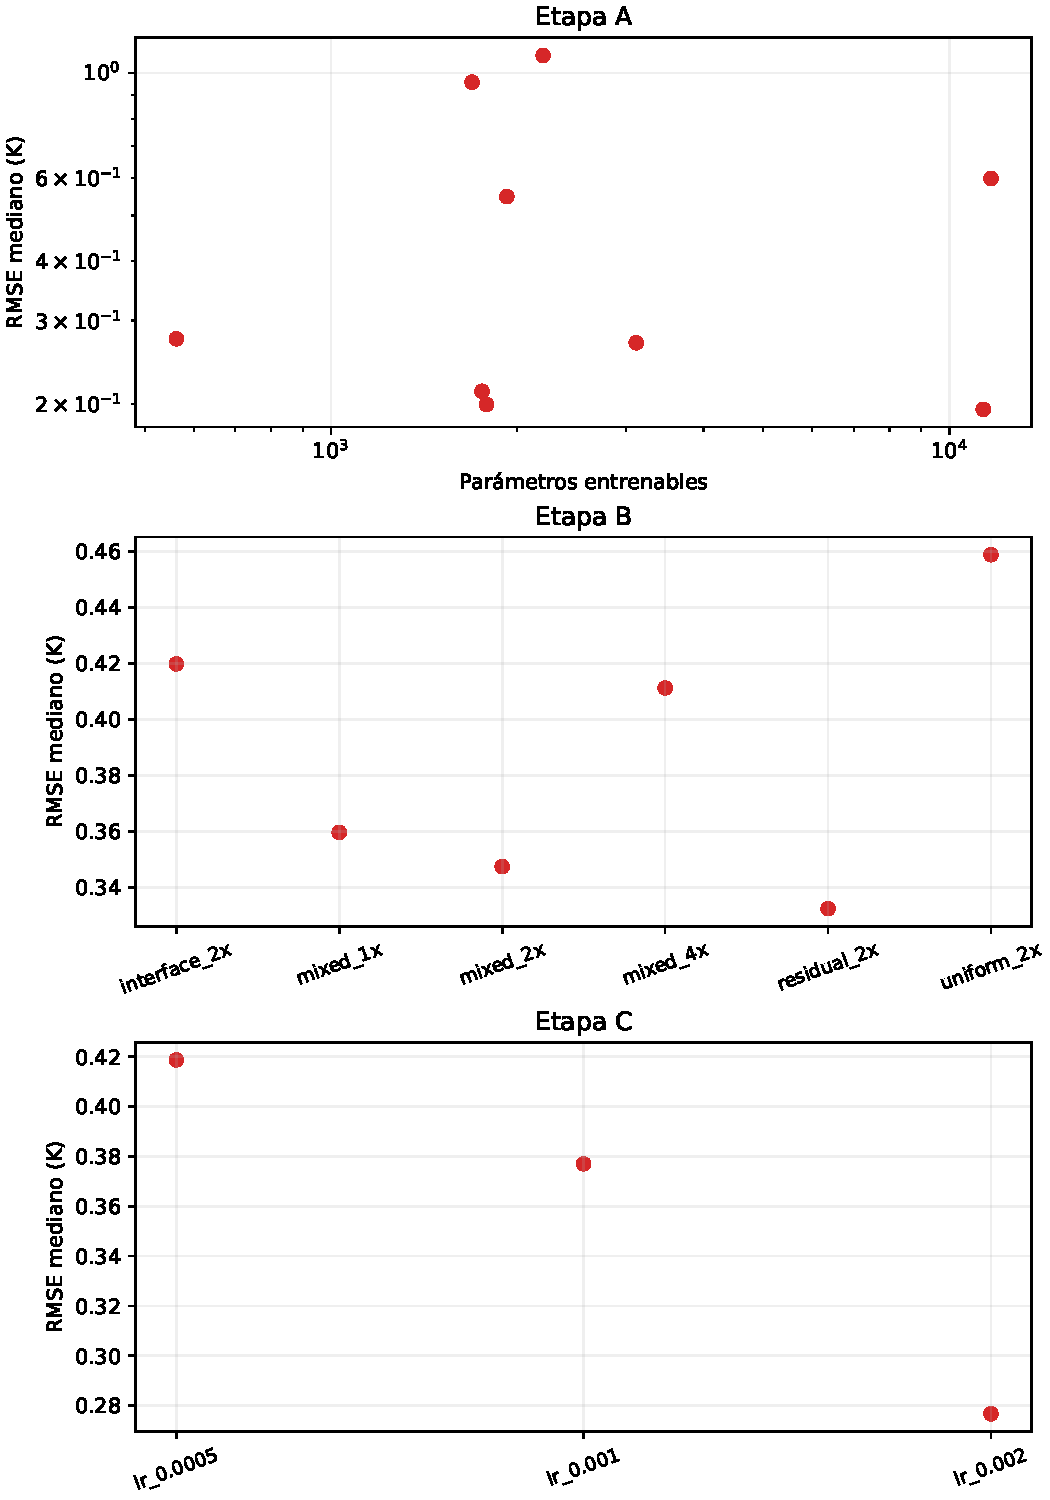
\includegraphics[width=.88\textwidth,height=.82\textheight,keepaspectratio]{explicit/selection.pdf}

\caption{Comparación de desarrollo. Verde: aceptación completa; rojo: al menos un rechazo. Los paneles corresponden a etapas distintas y no a un único factorial. Fuente: elaboración propia.}\end{figure}

\begin{figure}[htbp]\centering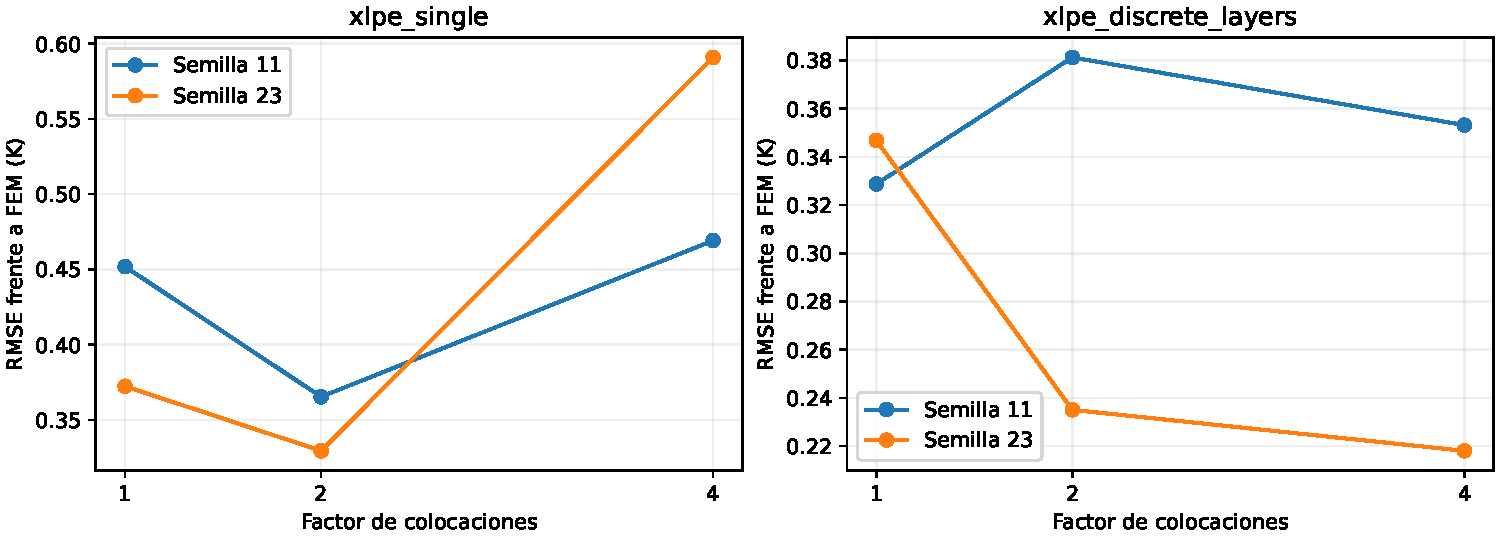
\includegraphics[width=\textwidth]{explicit/convergence.pdf}

\caption{Sensibilidad al número de colocaciones con la misma arquitectura y política geométrica. Fuente: elaboración propia.}\end{figure}

\begin{figure}[p]\centering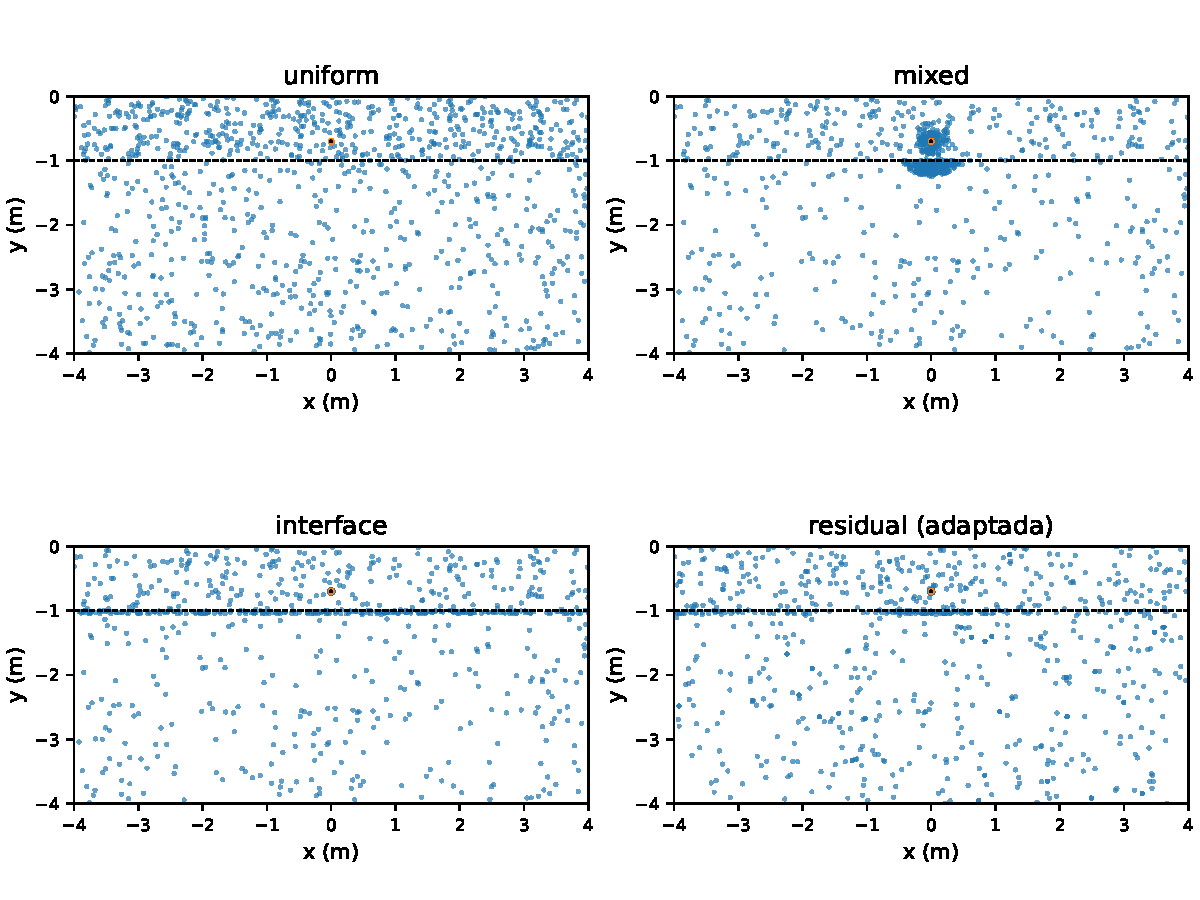
\includegraphics[width=\textwidth]{explicit/collocation_domain.pdf}

\caption{Cobertura del dominio para las cuatro políticas a igual presupuesto 2x, estratos y semilla 11. Azul: suelo; naranja: materiales del cable; líneas: interfaces geométricas. Se muestran colocaciones interiores, no las cuadraturas de trazas. Fuente: nubes archivadas; la política residual muestra la nube posterior a la adaptación.}\end{figure}

\begin{figure}[p]\centering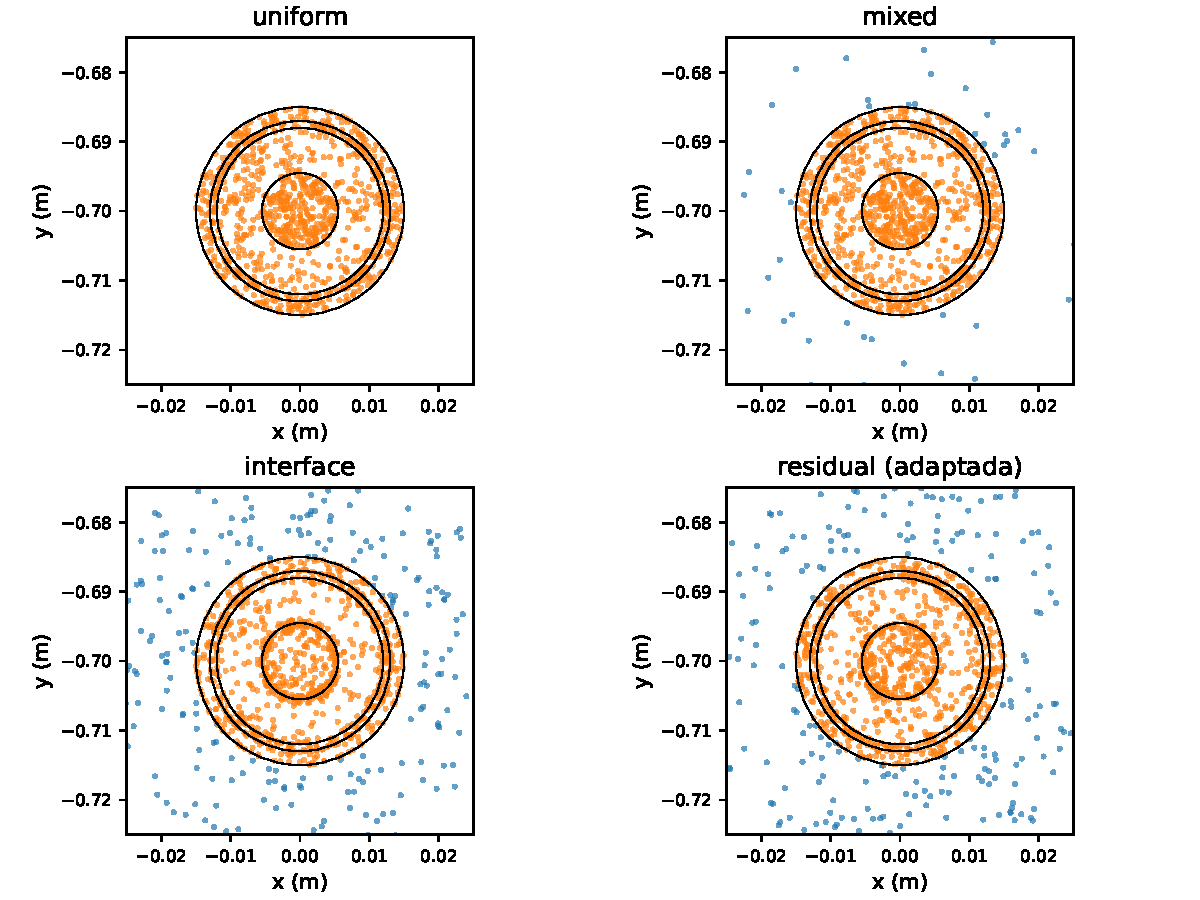
\includegraphics[width=\textwidth]{explicit/collocation_detail.pdf}

\caption{Detalle del cable para las cuatro políticas a igual presupuesto 2x, estratos y semilla 11. Azul: suelo; naranja: materiales del cable; líneas: interfaces geométricas. Se muestran colocaciones interiores, no las cuadraturas de trazas. Fuente: nubes archivadas; la política residual muestra la nube posterior a la adaptación.}\end{figure}

\begin{figure}[htbp]\centering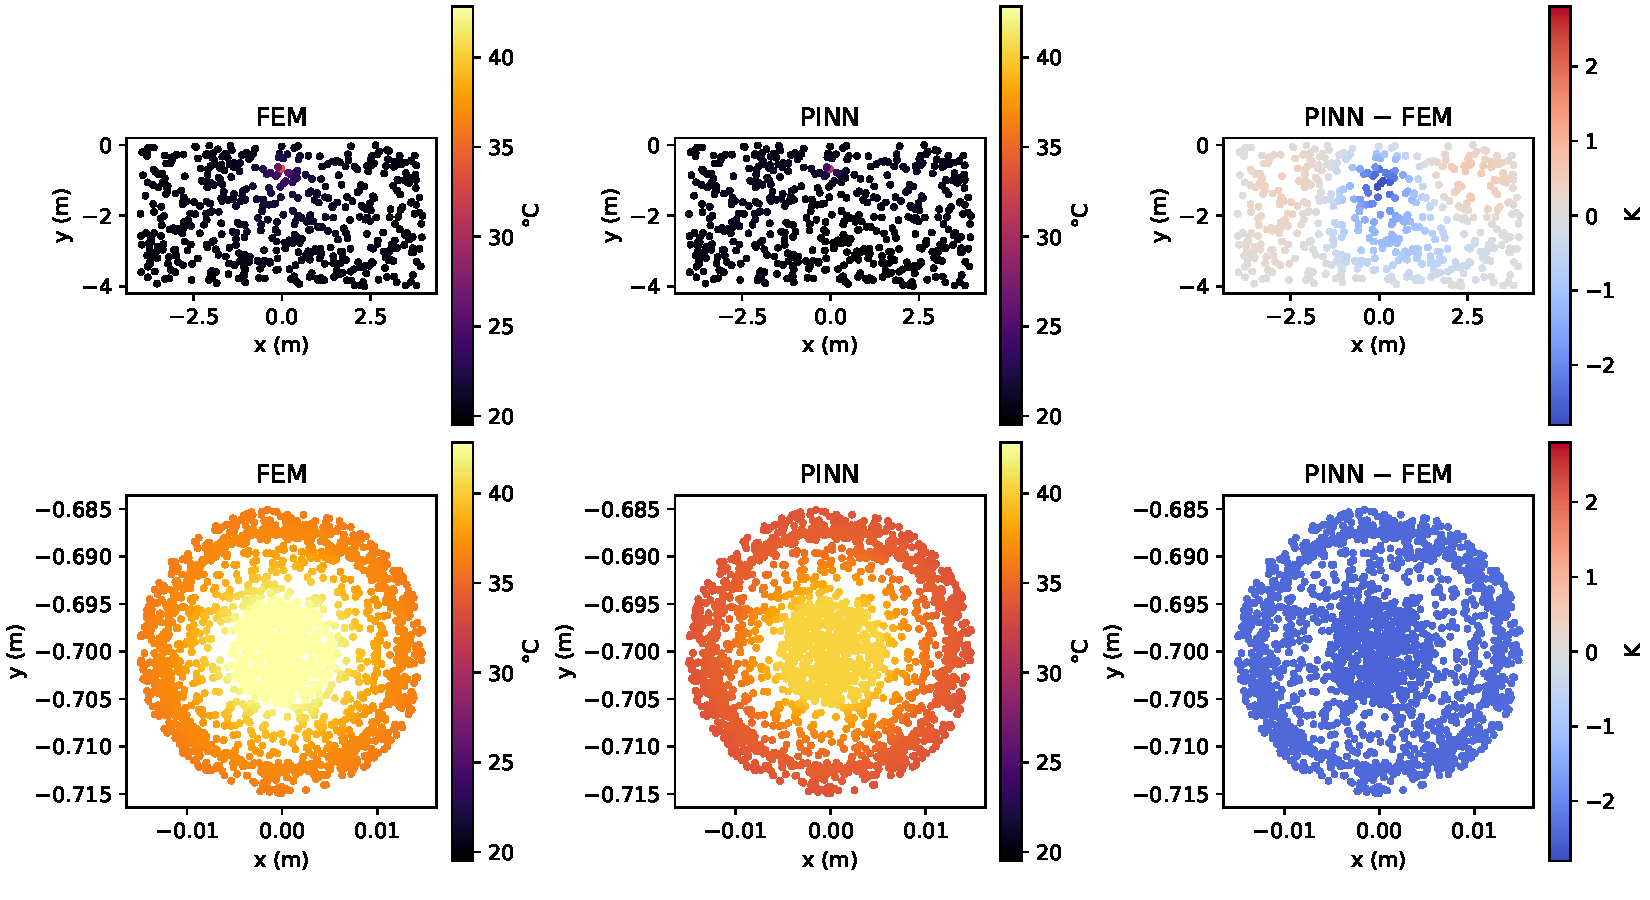
\includegraphics[width=\textwidth]{explicit/field.pdf}

\caption{Suelo y detalle interior del cable en XLPE con zona seca cercana, semilla 71 fijada previamente. Las temperaturas comparten escala y el error usa escala simétrica. Fuente: campos de confirmación.}\end{figure}


\subsection{EFECTO PIEL Y DISTRIBUCIÓN INTERIOR DEL CALOR}

El cálculo cilíndrico condicional, suponiendo R20 DC y conductor macizo homogéneo aislado, estima un incremento de pérdidas de 0,195--0,317\,\pct{} para el conductor XLPE pequeño y de 25,578--37,136\,\pct{} para los conductores grandes del catálogo, entre 90 y 20 °C. Estas cifras no certifican la resistencia AC de los cables publicados: construcción, frecuencia, temperatura y naturaleza del dato requieren procedencia primaria.

La comparación FEM 2D del caso Aras a igual potencia AC utilizó cuatro mallas por perfil de fuente. El cambio de Tmax al pasar de fuente uniforme a perfil piel fue $-0,004132$, $-0,004051$, $-0,004045$ y $-0,004045$ K. La malla fina tiene 380113 grados de libertad y balance de 0,002402\,\pct{}. La diferencia entre las dos últimas estimaciones del efecto es aproximadamente $4,1\times10^{-7}$ K. Se normalizó la fuente interpolada por su integral para impedir que un pequeño cambio de potencia contaminara la comparación de perfiles.

Este ensayo respalda que la redistribución radial resulta secundaria para la temperatura estacionaria de ese caso, frente al criterio de 0,1 K adoptado. No permite omitir el aumento de pérdidas AC ni extender la conclusión a proximidad, conductores segmentados o transitorios. La fuente no uniforme permanece disponible para todas las variantes y la conducción interior se resuelve siempre mediante la PDE.

\subsection{ACOPLAMIENTO LOCAL Y ALCANCE DE LA AMPACIDAD}

La formulación DC local se verificó en el caso coaxial con FEM y PINN explícitos: la referencia fina obtuvo 32,571582 °C y la PINN 32,575572 °C, diferencia de 0,003990 K. Este piloto demuestra la ejecución de la ley local de la Fórmula~\ref{for:fuente-dc-local}; no sustituye una campaña de confirmación de ampacidad. Las capacidades térmicas y las condiciones iniciales aún no se han utilizado para resolver una evolución temporal completa.

La búsqueda de corriente límite con la formulación explícita no se ha ejecutado y permanece pendiente. OE4 no se considera concluido con resultados de potencia fija ni con los de la formulación reducida anterior.


\subsection{DIAGNÓSTICO DE LOS RECHAZOS}
\label{sec:diagnostico-rechazos}

Un rechazo indica que algún criterio no se cumplió, pero no dice cuál limita cada problema. Para cada corrida se calcula la razón entre el valor observado y su tolerancia, con los mismos umbrales de la Sección~\ref{sec:seleccion-pinn}: \emph{campo} es el mayor entre el NRMSE global y el RMSE por material, frente a 5\,\pct{}; $T_{\max}$ es el error de la temperatura máxima, frente a 5\,\pct{}; \emph{energía} es el mayor desequilibrio global o regional, frente a 2\,\pct{}; \emph{salto de $T$} es el mayor salto de temperatura en una interfaz, frente a 0,1 K; y \emph{salto de flujo} es el mayor salto RMS de flujo normal, frente a 1\,\pct{}. Un valor mayor que 1 incumple el criterio. La Tabla~\ref{tab:explicit-D-diagnosis} muestra el máximo entre las tres semillas de confirmación para cada problema.

\begin{table}[htbp]
\centering
\caption{Etapa D: razón máxima entre el valor observado y la tolerancia, por criterio y problema (máximo entre las tres semillas). Un valor mayor que 1 incumple el criterio. Fuente: elaboración propia a partir de los registros de confirmación.}
\label{tab:explicit-D-diagnosis}
\setlength{\tabcolsep}{3pt}
\begin{tabularx}{\textwidth}{L{3.2cm}C{1.1cm}C{1.3cm}C{1.1cm}C{1.5cm}C{1.3cm}C{1.4cm}Y}
\toprule
Problema & Acept. & Campo & $T_{\max}$ & Energía & Salto de $T$ & Salto de flujo & Criterio dominante \\
\midrule
xlpe\_single & 3/3 & 0,45 & 0,45 & 0,44 & 0,31 & 0,55 & Ninguno \\
xlpe\_dry\_far & 3/3 & 0,52 & 0,52 & 0,48 & 0,27 & 0,53 & Ninguno \\
xlpe\_dry\_near & 1/3 & 2,16 & 2,16 & 0,86 & 0,40 & 0,59 & $T_{\max}$ y campo \\
xlpe\_backfill & 0/3 & 1,99 & 1,99 & 1,46 & 0,28 & 0,95 & $T_{\max}$ y campo \\
xlpe\_discrete\_layers & 0/3 & 0,92 & 0,92 & 0,52 & 1,70 & 1,88 & Salto de flujo y de $T$ \\
aras\_flat & 0/3 & 16,21 & 5,54 & 0,12 & 1,18 & 0,59 & Campo \\
kim\_sand & 0/3 & 6,29 & 5,75 & 1,34 & 2,51 & 2,02 & Campo y $T_{\max}$ \\
\bottomrule
\end{tabularx}
\end{table}

Los rechazos tienen causas distintas. En Aras plano y en Kim en arena el campo supera varias veces la tolerancia (16,21 y 6,29 en la peor semilla): la red no reproduce el campo, y en Kim también se incumplen ambos saltos de interfaz. En el relleno y en la zona seca cercana el error de $T_{\max}$ llega a 1,99 y 2,16 veces la tolerancia, cerca del umbral; en la zona seca cercana la semilla 83 sí cumplió (0,76), de modo que el resultado no es reproducible. En los estratos, el campo y $T_{\max}$ quedan dentro de la tolerancia (0,92) y el rechazo procede solo de la continuidad en la interfaz: un salto RMS de flujo de 1,88\,\pct{} y un salto de temperatura de 0,17 K, frente a 1\,\pct{} y 0,1 K. Estas razones indican qué criterio limita cada problema con el presupuesto usado; no demuestran que la arquitectura sea incapaz de cumplirlo.

La misma lectura se aplica al ajuste. La Tabla~\ref{tab:explicit-C-diagnosis} muestra que en C el salto de temperatura en las interfaces fue el criterio dominante para las tres tasas de aprendizaje (4,4 a 5,1 veces la tolerancia), mientras que campo y $T_{\max}$ quedaron por debajo de 1. En C2, aumentar $w_T$ redujo ese salto, pero desplazó la restricción al flujo: con $w_T=1000$ el salto de temperatura fue 1,60 y el de flujo 1,56; con $w_T=10000$, 0,23 y 2,07. Ningún candidato cumplió todos los criterios en las cuatro corridas de desarrollo, de modo que la receta congelada ($w_T=1000$, tasa $5\times10^{-4}$) es la mejor según la regla declarada y no una receta demostrada. El compromiso entre continuidad de temperatura y de flujo reaparece en los estratos de D.

\begin{table}[htbp]
\centering
\caption{Etapas C y C2: razón máxima entre el valor observado y la tolerancia, por candidato (máximo entre las cuatro corridas de desarrollo). El candidato $w_T=100$ de C2 reutiliza las corridas de C con tasa $5\times10^{-4}$. Fuente: elaboración propia a partir de los registros de desarrollo.}
\label{tab:explicit-C-diagnosis}
\setlength{\tabcolsep}{3pt}
\begin{tabularx}{\textwidth}{L{3.2cm}C{1.1cm}C{1.3cm}C{1.1cm}C{1.5cm}C{1.3cm}C{1.4cm}Y}
\toprule
Etapa y candidato & Acept. & Campo & $T_{\max}$ & Energía & Salto de $T$ & Salto de flujo & Criterio dominante \\
\midrule
C, tasa $5\times10^{-4}$ ($w_T=100$) & 2/4 & 0,71 & 0,67 & 0,45 & 4,49 & 1,22 & Salto de $T$ \\
C, tasa $10^{-3}$ & 1/4 & 0,70 & 0,69 & 0,43 & 4,42 & 1,07 & Salto de $T$ \\
C, tasa $2\times10^{-3}$ & 1/4 & 0,52 & 0,22 & 0,30 & 5,13 & 1,15 & Salto de $T$ \\
C2, $w_T=1000$ & 2/4 & 0,80 & 0,80 & 0,43 & 1,60 & 1,56 & Salto de $T$ \\
C2, $w_T=10000$ & 2/4 & 0,57 & 0,57 & 0,35 & 0,23 & 2,07 & Salto de flujo \\
\bottomrule
\end{tabularx}
\end{table}

\subsection{DOMINIO DE ACEPTACIÓN}
\label{sec:dominio-validez}

El dominio de aceptación es el conjunto de problemas para los que la receta congelada cumplió todos los criterios con las tres semillas de confirmación. La Tabla~\ref{tab:dominio-aceptacion} lo fija con la evidencia de D. Un problema aceptado lo está para su geometría, su fuente prescrita y su contorno de 20 °C en el dominio de 8×4 m, con reentrenamiento por caso; la aceptación no se transfiere a otras geometrías, a otras propiedades ni a redes ya entrenadas.

\begin{table}[htbp]
\centering
\caption{Dominio de aceptación de la receta congelada según la confirmación con semillas nuevas. Fuente: elaboración propia a partir de la Tabla~\ref{tab:explicit-production} y del diagnóstico de la Sección~\ref{sec:diagnostico-rechazos}.}
\label{tab:dominio-aceptacion}
\begin{tabularx}{\textwidth}{L{3.4cm}C{1.5cm}L{2.6cm}Y}
\toprule
Problema & Semillas aceptadas & Estado & Condición de uso \\
\midrule
xlpe\_single & 3/3 & Aceptado & Un cable XLPE en suelo homogéneo, con fuente prescrita. \\
xlpe\_dry\_far & 3/3 & Aceptado & Igual, con zona seca de $k=0,5$ W/(m K) a 1 m del eje. \\
xlpe\_dry\_near & 1/3 & Restringido & Resultado no reproducible entre semillas; requiere verificación con FEM antes de cualquier uso. \\
xlpe\_backfill & 0/3 & No aceptado & Candidato a la ronda E. \\
xlpe\_discrete\_layers & 0/3 & No aceptado & Candidato a la ronda E; el límite es la continuidad en la interfaz. \\
aras\_flat & 0/3 & No aceptado & No se reabre sin un cambio de arquitectura o de presupuesto que se justifique. \\
kim\_sand & 0/3 & No aceptado & Igual que Aras plano. \\
\bottomrule
\end{tabularx}
\end{table}

La \emph{ronda E} es una ronda de desarrollo preinscrita, no ejecutada. Se propone para los estratos, el relleno y la zona seca cercana, con semillas nuevas y con los mismos criterios de aceptación, de modo que no se modifiquen los umbrales después de observar resultados. Su protocolo (casos, cambios permitidos a la receta, semillas, regla de parada y reporte íntegro de las corridas) se registra en el archivo \texttt{docs/PROTOCOLO\_RONDA\_E.md} del repositorio y debe aprobarse antes de ejecutarla. Hasta que se ejecute, el dominio aceptado es el de la Tabla~\ref{tab:dominio-aceptacion}. Ejecutarla exige entrenamientos nuevos; por ello queda como trabajo pendiente y no como resultado de la investigación.

\subsection{MATRIZ DE VALIDEZ}
\label{sec:matriz-validez}

La Tabla~\ref{tab:matriz-validez} separa lo que la evidencia verifica, contra qué referencia y lo que no establece. Su función es evitar que una aceptación numérica se lea como validación de una instalación real.

\begin{table}[htbp]
\centering
\caption{Matriz de validez de la evidencia. Fuente: elaboración propia a partir de las Tablas~\ref{tab:explicit-fem}, \ref{tab:explicit-production}, \ref{tab:explicit-effects} y~\ref{tab:explicit-effect-resolution}.}
\label{tab:matriz-validez}
\setlength{\tabcolsep}{3pt}
\begin{tabularx}{\textwidth}{L{2.7cm}Y Y Y}
\toprule
Qué se verifica & Contra qué referencia & Evidencia obtenida & Qué no establece \\
\midrule
Referencia FEM & Tres mallas por caso; cambio de $T_{\max}$ menor a 0,1 K y balance menor a 0,2\,\pct{} entre las dos últimas. & Mayor cambio de $T_{\max}$: 0,078 K; mayor balance: 0,027\,\pct{} (Tabla~\ref{tab:explicit-fem}). & Una cota del error exacto; propiedades reales, contornos o extensión del terreno. \\
Código FEM en simetría radial & Solución analítica coaxial. & Error de $T_{\max}$ de aproximadamente $3{,}68\times10^{-6}$ K. & Los casos angulares y heterogéneos. \\
Aceptación de la PINN & FEM de la misma formulación en puntos idénticos; seis criterios de la Sección~\ref{sec:seleccion-pinn}. & 7 de 21 ejecuciones aceptadas (Tabla~\ref{tab:explicit-production}). & Generalización a otros casos o a otras semillas; equivale a reentrenar por caso. \\
Efecto térmico de la heterogeneidad & Pares frente al XLPE homogéneo, a igual fuente prescrita. & Diferencias de $T_{\max}$ por caso (Tabla~\ref{tab:explicit-effects}). & Un efecto concluyente: ninguno satisfizo la regla de resolución preinscrita (Tabla~\ref{tab:explicit-effect-resolution}). \\
Contraste con valores publicados & Las geometrías de Aras (2005) y Kim (2025) se adoptan solo como configuración. & No se ha realizado con la formulación explícita. & Concordancia con las temperaturas publicadas: exige reproducir sus pérdidas, propiedades y contornos. \\
Ampacidad explícita & Búsqueda de corriente límite con la misma ley de pérdidas. & No ejecutada. & Cumplimiento de OE4 en la formulación explícita. \\
Validez de campo & Mediciones de instalaciones reales. & No realizadas. & Comportamiento de una instalación real. \\
\bottomrule
\end{tabularx}
\end{table}

La comparación con valores publicados queda pendiente porque las temperaturas de la Tabla~\ref{tab:explicit-fem} para Aras plano y Kim en arena proceden de fuentes prescritas por cable, de $k$ base y de contornos del contrato de caso, que no coinciden con los de esas publicaciones. Compararlas directamente con las temperaturas publicadas sería una comparación entre problemas distintos.

\section{DISCUSIÓN E INTERPRETACIÓN}
\label{sec:discusion}

La pregunta principal es qué configuración satisface conjuntamente las ecuaciones, interfaces y referencia en el dominio ensayado. Una pérdida menor, un campo visualmente suave o una Tmax cercana no constituyen por sí solos aceptación. Los resultados negativos de redes pequeñas delimitan su utilidad con el presupuesto empleado, sin demostrar que una red mayor sea siempre preferible.

La selección secuencial permite estudiar decisiones concretas con un coste limitado, pero omite interacciones entre arquitectura, muestreo y entrenamiento. Una arquitectura descartada en A podría mejorar con otra distribución o presupuesto. Los resultados se interpretan como búsqueda preliminar controlada, no como optimización global ni clasificación universal de familias PINN. Las semillas pareadas reducen diferencias de diseño entre alternativas, pero dos o tres semillas no bastan para estimar colas de fallo poco frecuentes.

La referencia FEM también tiene error y depende de propiedades y contornos. Las pruebas de malla y el control analítico reducen incertidumbre numérica, sin validar una instalación. La incertidumbre de k, resistencia, contactos, pérdidas y humedad no se convierte en incertidumbre estadística mediante variación de semillas. Las inferencias sobre heterogeneidad se limitan a pares donde la diferencia física supera el cambio de discretización y la dispersión de los solucionadores aceptados.

Los resultados de la confirmación admiten tres lecturas. Primero, la receta es reproducible en los problemas más simples: el XLPE homogéneo y la zona seca lejana se aceptaron en las tres semillas. Segundo, la aceptación desaparece con interfaces exigentes y con arreglos de varios cables. El diagnóstico de la Sección~\ref{sec:diagnostico-rechazos} muestra que en los estratos el límite es la continuidad de flujo y de temperatura; en el relleno y la zona seca cercana, un error de $T_{\max}$ próximo al umbral; y en Aras y Kim, el error de campo. Tercero, las diferencias de temperatura respecto al control homogéneo (Tabla~\ref{tab:explicit-effects}) no alcanzan la regla de resolución preinscrita (Tabla~\ref{tab:explicit-effect-resolution}), por lo que no se interpretan como efectos térmicos de la heterogeneidad.

Por ello el resultado es una aceptación acotada al dominio de la Tabla~\ref{tab:dominio-aceptacion} y no una demostración del enfoque para cables enterrados en general. El conteo de 7 aceptaciones en 21 ejecuciones no estima una probabilidad de éxito sobre una población de instalaciones: cada problema tiene tres semillas y fue elegido como caso de estudio, no muestreado de una población. La contribución de la ciencia del diseño es el procedimiento que hizo visible cada límite: especificar la misma física para PINN y FEM, exigir la transmisión de temperatura y de flujo en cada interfaz, comprobar el flujo calculado de $-k\nabla T$ y no solo el auxiliar, fijar los umbrales antes de confirmar y conservar los rechazos. Ese procedimiento también indica qué cambiar en la ronda E y qué no reabrir sin una razón nueva.

El alcance temporal sigue siendo una extensión: disponer del operador $\rho c_pT_t$ no demuestra un solucionador transitorio verificado. La ampacidad normativa AC requiere pérdidas dieléctricas, pantallas, proximidad y condiciones de instalación que exceden los controles ejecutados. Las conclusiones de OE4 deben basarse en una búsqueda de corriente límite de la formulación explícita y no en tablas heredadas del modelo reducido.

\section{IMPACTO Y PRODUCTO REPRODUCIBLE}
\label{sec:impacto}

El impacto demostrado es metodológico y computacional: especificar una física común, detectar comparaciones incompatibles, seleccionar una receta con reglas previas, repetirla con semillas nuevas y conservar tanto aceptaciones como rechazos. El impacto profesional potencial consiste en identificar casos que merecen evaluación térmica detallada. No se afirman ahorros, incremento autorizado de capacidad ni superioridad temporal sobre FEM sin evidencia específica.

\subsection{VIABILIDAD TÉCNICA Y COSTO COMPUTACIONAL}

La viabilidad se evalúa con lo que registró la campaña. La Tabla~\ref{tab:costo-computacional} resume el costo de una corrida de confirmación por problema: entre 8 y 11 minutos para el XLPE de un cable, 21 minutos para Aras plano y 92 minutos para Kim en arena, que es el problema con más parámetros y más capas. Las 101 corridas de las etapas A a D sumaron 15,0 horas de tiempo de corrida, de las cuales 8,0 horas corresponden a D. Se ejecutaron en un equipo con CPU Intel Core Ultra 7 165U, sin CUDA, en precisión doble y con hasta tres procesos concurrentes, de modo que esa suma sobrestima el tiempo transcurrido. Los tiempos concurrentes compiten por recursos y no se comparan con FEM: no se midió el tiempo de FEM en condiciones equivalentes y la tesis no afirma ventaja ni desventaja temporal.

\begin{table}[htbp]
\centering
\caption{Costo computacional por corrida de confirmación (etapa D, tres semillas por problema). Fuente: elaboración propia a partir de los registros de confirmación.}
\label{tab:costo-computacional}
\begin{tabularx}{\textwidth}{L{3.6cm}C{2.2cm}C{1.7cm}C{1.7cm}C{1.7cm}Y}
\toprule
Problema & Parámetros entrenables & Mínimo, s & Mediana, s & Máximo, s & Aceptadas \\
\midrule
xlpe\_single & 11338 & 496 & 505 & 505 & 3/3 \\
xlpe\_dry\_far & 11338 & 528 & 532 & 537 & 3/3 \\
xlpe\_dry\_near & 11338 & 513 & 514 & 516 & 1/3 \\
xlpe\_backfill & 11338 & 510 & 511 & 523 & 0/3 \\
xlpe\_discrete\_layers & 13612 & 656 & 672 & 675 & 0/3 \\
aras\_flat & 29530 & 1277 & 1278 & 1303 & 0/3 \\
kim\_sand & 125038 & 5487 & 5546 & 5560 & 0/3 \\
\bottomrule
\end{tabularx}
\end{table}

El costo por resultado aceptado es más informativo que el costo por corrida. En D se aceptaron 7 de 21 ejecuciones y más de dos tercios de las horas se gastaron en Aras y Kim, donde no se aceptó ninguna. Un problema mayor exige más parámetros y más tiempo, pero la evidencia muestra que más recursos no garantizan aceptación; el resultado depende del criterio que limita cada caso (Sección~\ref{sec:diagnostico-rechazos}).

\subsection{RIESGOS Y BENEFICIO--COSTO}

La Tabla~\ref{tab:matriz-riesgos} resume los riesgos identificados, con probabilidad e impacto cualitativos y la mitigación adoptada o pendiente.

\begin{table}[htbp]
\centering
\caption{Matriz cualitativa de riesgos del artefacto y de su uso. Fuente: elaboración propia a partir de los resultados de la campaña.}
\label{tab:matriz-riesgos}
\begin{tabularx}{\textwidth}{L{3.6cm}C{1.8cm}C{1.5cm}Y}
\toprule
Riesgo & Probabilidad & Impacto & Mitigación \\
\midrule
Rechazo del artefacto en configuraciones de interés (7 de 21 ejecuciones aceptadas). & Alta & Alto & Declarar el dominio de aceptación; ejecutar la ronda E; verificar con FEM antes de usar. \\
Uso fuera del dominio aceptado como si fuera una certificación. & Media & Alto & La etiqueta ``producción'' no certifica; la matriz de validez y la conservación de rechazos delimitan el uso. \\
Variabilidad entre semillas con solo dos o tres repeticiones. & Media & Medio & Informar mediana, rango y cantidad aceptada; confirmar con semillas nuevas. \\
Costo de los problemas grandes (Kim, 92 minutos por corrida). & Media & Medio & Presupuestos declarados; no ampliar sin una razón física o numérica. \\
Cambios de versión del software (FEniCSx, Gmsh, PyTorch). & Media & Medio & Versiones y huellas registradas en cada expediente; fijar rangos de dependencias queda pendiente. \\
Leer la ampacidad no ejecutada como resultado. & Media & Alto & OE4 se declara no alcanzado en la formulación explícita; no se afirma corriente admisible. \\
\bottomrule
\end{tabularx}
\end{table}

El beneficio es principalmente metodológico: un procedimiento trazable, criterios de aceptación reutilizables, un dominio delimitado y una base para decidir cuándo una PINN no debe usarse sin verificación con FEM. Los costos son las horas de cómputo (15,0 horas de tiempo de corrida en la campaña), el trabajo de preparar referencias FEM verificadas para cada caso y la necesidad de reentrenar la red por problema. El balance es cualitativo: el beneficio se apoya en la calidad y en la trazabilidad del procedimiento y no en un ahorro económico o de tiempo, que no se estimó.

\subsection{SOSTENIBILIDAD}

El estudio se autofinancia y emplea software de código abierto (FEniCSx, Gmsh, PETSc y PyTorch), por lo que no requiere licencias comerciales. El consumo eléctrico de la campaña no se midió y no se hacen afirmaciones sobre él. La mantenibilidad depende de que los expedientes conserven versiones, huellas y configuraciones; la definición de licencia del repositorio y el acotamiento de las versiones de las dependencias son tareas pendientes.
